\documentclass[10pt]{article}
\usepackage{zpj}
\usepackage{amsthm}
\usepackage{braket}
\usepackage{hyperref}
\title{Global optimization}
\author{Peijun Zhu}
\newtheorem{theorem}{Theorem}[section]
\begin{document}
\maketitle
\section{Derivatives over a small perturbation}
\subsection{Basic Derivatives}
Define function $f$ as the expectation value of Hermitian operator $h$ with density matrix $\rho$ transformed by $U=\ee^{\ii xM}$:
\begin{equation}
f(xM, h, \rho)=\tr \Big[\ee^{\ii xM}\rho \ee^{-\ii xM}h\Big],
\end{equation}
where $M$ is a nonzero Hermitian operator defining the direction of optimization. 

At $x=0$, the directional derivative
\[\frac{\pp f}{\pp x}\Big|_{x=0}=\tr \Big[M\ii [\rho, h]\Big]\mdef [M, \rho, h],\]
where $[\cdot, \cdot, \cdot]$ is tri-linear and antisymmetric.
\begin{align}
\frac{\pp^2 f}{\pp x^2}\Big|_{x=0}&=\tr \Big[2M\rho Mh-M^2\rho h-\rho M^2h\Big]\\
&=\tr \Big[[M,\rho][M, h]\Big]\\
&=2\tr \Big[M\rho [M, h]\Big]=2\tr \Big[Mh [M, \rho]\Big]
\end{align}

In conclusion, we have Taylor expansion
\[f= \tr[\rho h] + \tr\Big[M\ii[\rho, h]\Big]x + \tr \Big[[M,\rho][M, h]\Big]\frac{x^2}{2}+O(x^3) \]

Any Hermitian matrix $M$ can be expanded by some linear independent bases matrix, i.e.\ $M=\sum x_iM_i$, with gradient and Hessian 
\begin{equation}
\nabla_i f=[M_i,\rho, h], \quad H_{ij}f=2\tr \Big[M_i\rho[M_j, h]\Big]
\end{equation}

\subsection{Derivatives of variance}
For given $H$, variance $V$ of energy for $\rho$ under a small unitary transformation $\ee^{\ii xM}$ is 
\begin{equation}
V(xM)=\langle H^2\rangle(xM)-\langle H\rangle^2(xM)=f(xM, H^2, \rho)-f^2(xM, H, \rho)
\end{equation}
From the chain rule, we have
\begin{align}
\frac{\pp V}{\pp x}\Big|_{x=0}&=\frac{\pp \langle H^2\rangle}{\pp x}-2\langle H\rangle\frac{\pp \langle H\rangle}{\pp x}\Big|_{x=0}\\
&=[M, \rho, H^2]-2E[M, \rho, H]\\
&= [M, \rho, (H-E)^2]
\end{align}
\begin{align}
\frac{\pp^2 V}{\pp x^2}\Big|_{x=0}&=\frac{\pp^2 \langle H^2\rangle}{\pp x^2}-2\langle H\rangle\frac{\pp^2 \langle H\rangle}{\pp x^2}-2\left(\frac{\pp \langle H\rangle}{\pp x}\right)^2\Big|_{x=0}\\
&=\tr \Big[[M,\rho][M, H^2]\Big]-2E\tr \Big[[M,\rho][M, H]\Big]-2[M, \rho, H]^2\\
&=\tr \Big[[M,\rho][M, H^2-2EH]\Big]-2[M, \rho, H]^2\\
&=\tr \Big[[M,\rho]\big[M, (H-E)^2\big]\Big]-2[M, \rho, H]^2
\end{align}
\begin{equation}
	H_{ij}=\tr \Big[[M_i,\rho]\big[M_j, (H-E)^2\big]\Big]-2[M_i, \rho, H][M_j, \rho, H]
\end{equation}
\section{Stationary points (\texorpdfstring{$[\rho, (H-E)^2]=0$}{[rho, (H-E)**2]=0})}
If variance $V$ reaches a stationary point, where $\pp V/\pp x|_{x=0}\equiv 0$ for any $M$, we can prove $[\rho, (H-E)^2]=0$. We want to prove that those stationary points $[\rho, (H-E)^2]=0$ without condition $[\rho, H]= 0$ are not local minimum points. 

Generally, any $M$ satisfying $[M, (H-E)^2]=0$ make $V'$ and first term in $V''$ vanish. As $[\rho, H]\neq 0$, we can choose $M_0=\ii[\rho, H]$ as the generator of unitary transformation. As both $\rho$ and $H$ commutes with $(H-E)^2$, it is obvious that $[M_0, (H-E)^2]=0$. For $M_0$
\begin{equation}
\frac{\pp V}{\pp x}\Big|_{x=0}=0,\quad \frac{\pp^2 V}{\pp x^2}\Big|_{x=0}=-2\big|[\rho, H]\big|^2<0,
\end{equation}
where $|\cdot|$ is the Frobenius norm of matrix. 

\section{Stationary points with \texorpdfstring{$[\rho, H]=0$}{[rho, H]=0}}
Even for $[\rho, H]=0$, it may still be a saddle point. In this section, we are giving a equivalent criteria for minimum points. If $[\rho, H]=0$, then $[\rho, (H-E)^2]=0$ and
\begin{equation}
\pp V/\pp x|_{x=0}\equiv 0,\quad \pp^2 V/\pp x^2|_{x=0}=\tr \Big[[M,\rho]\big[M, (H-E)^2\big]\Big]
\end{equation}
It is obvious that for any $M$ diagonal in CSCO(Complete Set of Commuting Observables) of $\rho$ and $H$, transformation $\ee^{\ii M}$ does not change $\rho$. So we only consider diagonal free $M$. For elementary $M_{ij}$ in subspace of $\ket{i}$ and $\ket{j}$:
\[M_{ij}\mdef m_{ij}\ket i\bra j+m_{ji}\ket j\bra i\]
If we define $\Delta_k=E_k-E$, then 
\begin{align}
V''(M_{ij})&=\tr \Bigg[\begin{bmatrix}
0 &-m_{ij}(\rho_i-\rho_j)\\
m_{ji}(\rho_i-\rho_j) &0
\end{bmatrix}\begin{bmatrix}
0 &-m_{ij}(\Delta_i^2-\Delta_j^2)\\
m_{ji}(\Delta_i^2-\Delta_j^2) &0
\end{bmatrix}\Bigg]\\
&=-2|m_{ij}|^2(\rho_i-\rho_j)(\Delta_i^2-\Delta_j^2)\label{deriv}
\end{align}

\begin{theorem}
\begin{equation}
(\rho_i-\rho_j)(\Delta_i^2-\Delta_j^2)\leq0,\quad \forall i,j\label{rho}
\end{equation}
is sufficient and necessary condition for 
\begin{equation}V''\geq 0,\quad \forall M\label{allm}\end{equation}
\end{theorem}

\begin{proof}

\emph{Necessity}: If $V''\geq 0$ for any $M$, we must have $V''(M_{ij})\geq 0$. Then \ref{deriv} conveniently gives \ref{rho}.

\emph{Sufficiency}: If \ref{rho} is true then all $V''(M_{ij})>0$. Any $M$ can be decomposed into sum of $M_{ij}$, i.e.\ $M=\sum_{i<j} M_{ij}$. They have derivatives
\begin{align}
	V''(M)&=\sum_{i<j}\sum_{k<l}\tr \Big[[M_{ij},\rho]\big[M_{kl}, (H-E)^2\big]\Big]\\
	&=\sum_{i<j} \Big[[M_{ij},\rho]\big[M_{ij}, (H-E)^2\big]\Big]\\
	&=\sum_{i<j} V''(M_{ij})\\
	&\geq 0
\end{align}
\end{proof}

\noindent Likewise we can have
\begin{theorem}
\begin{equation}
	(\rho_i-\rho_j)(\Delta_i^2-\Delta_j^2)< 0,\; \forall i,j \quad \Leftrightarrow \quad V''>0,\;\forall M\label{rho2},
\end{equation}
\end{theorem}

\subsection{Conclusion}

Condition (\ref{rho}) is sufficient and necessary condition that $V''\geq 0$, i.e.\ Hessian is positive semidefinite. Similar condition (\ref{rho2}) is sufficient and necessary condition that $V''> 0$, i.e.\ Hessian is positive definite. This means that larger eigenvalues of $\rho$ should reside in eigenstate with energy close to mean energy, otherwise we can optimize the variance by applying $M_{ij}$ which swaps two eigenvalues of $\rho$. This is intuitive and also numerically confirmed.

Furthermore, there are possibly multiple local minimums, as these conditions does not guarantee uniqueness. As an simple example, for \[H_0=\diag[0,1,3],\quad\rho=\diag[1/6,1/3,1/2],\]there are two local minimum: $\rho_1=\diag[1/6,1/2,1/3]$ and $\rho_2=\diag[1/6,1/3,1/2]$
\begin{figure}[htb]
\centering
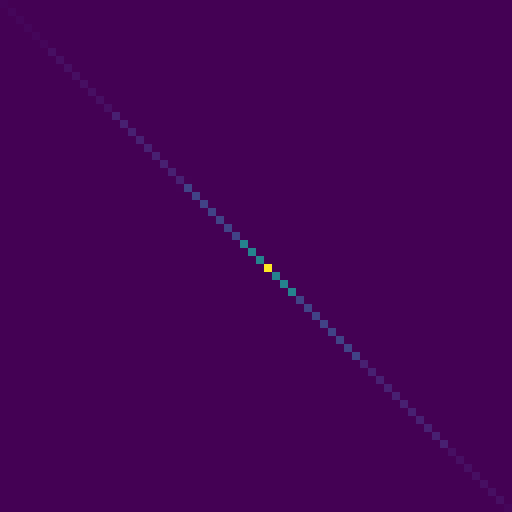
\includegraphics[height=5cm]{optimized.png}
\caption{$\rho$ in energy eigenbases}
\end{figure} 
\section{Optimization Process}
If $\big|[\rho, (H-E)^2]\big|>k\big|[\rho, H]\big|$, $k\sim\sqrt{V}$, we assume $\rho$ is not near a saddle point. In this case we can use $M=\ii[\rho, (H-E)^2]$ as optimization direction. If the condition is not satisfied, $M=\ii [\rho, H]$ may be a (temporary) better optimization direction. For every optimization step, if the initial step size $x$ does not really give a smaller variance, we try to half the step size iteratively. Optimization process terminates if there is no smaller variance. 
\end{document}